\newpage
\section{Part C}
\label{sec:sec_c}

Next, because we are using linear regression the dataset must be made linear. In order to do so, the natural log was taken of \textit{I}$_{d}$. Linear regression was than ran by manually computing the gradients as shown in the below code. Training lasted for $500$ epochs and has a learning rate of $0.01$. MSE was used to compute the loss and the loss curve is shown in Figure~\ref{fig:loss}. After training the final value of \textit{b} and \textit{w} were found to be $-15.2738$ and $15.5091$ respectively when unnormalized. The training loss for the final epoch was $0.001532$

\LST{part\_c}

\begin{figure}[!htpb]
	\centering
	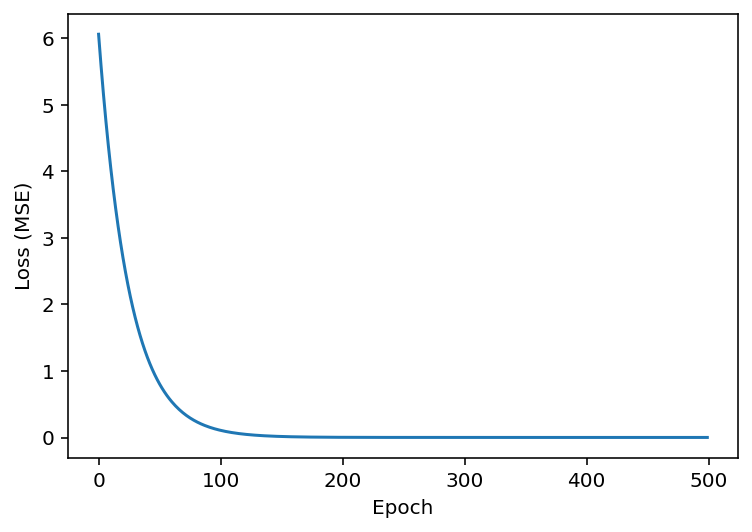
\includegraphics{figures/loss.png}
	\caption{Training Loss Curve}
	\label{fig:loss}
\end{figure}